\documentclass[11pt]{article}
\usepackage[margin=1in]{geometry}
\usepackage{amsmath,amssymb,amsthm}
\usepackage{graphicx}
\usepackage[hidelinks]{hyperref}

\newtheorem{theorem}{Theorem}
\newtheorem{corollary}{Corollary}
\newtheorem{remark}{Remark}

\newcommand{\R}{\mathbb R}
\newcommand{\N}{\mathbb N}
\newcommand{\OmegaN}{\omega_N}
\newcommand{\supp}{\operatorname{supp}}
\newcommand{\dist}{\operatorname{dist}}
\newcommand{\Lip}{\operatorname{Lip}}

\title{A Lipschitz Resolution of the Missing \(L^1\) Bound for Variable-Step Mollifiers}
\author{FA/Banach automatic math run}
\date{2026-07-18}

\begin{document}
\maketitle

\section*{Source And Target}

The source is Michael Hintermuller, Kostas Papafitsoros, and Carlos N.
Rautenberg, \emph{Variable step mollifiers and applications},
arXiv:1910.02751, published in \emph{Integral Equations and Operator Theory}
92 (2020), article 53.  For an open bounded set
\(\Omega\subset\R^N\), a non-negative compactly supported mollifier
\(\rho\) on the unit ball, and a variable step \(\eta\), the source studies
\[
  T_n f(x)=C_n(x)\int_\Omega
  \rho\left(\frac{x-y}{\eta(x)/n}\right) f(y)\,dy,
  \qquad
  C_n(x)=M_\rho \frac{n^N}{\eta(x)^N}.
\]
In Section 5, after proving the uniform \(L^1\) estimate under the quadratic
boundary condition
\[
  \kappa\,\dist(x,\partial\Omega)^2\le \eta(x)\le
  \dist(x,\partial\Omega)^2,
\]
the source asks whether the estimate remains true without imposing a condition
of that type.

\begin{center}
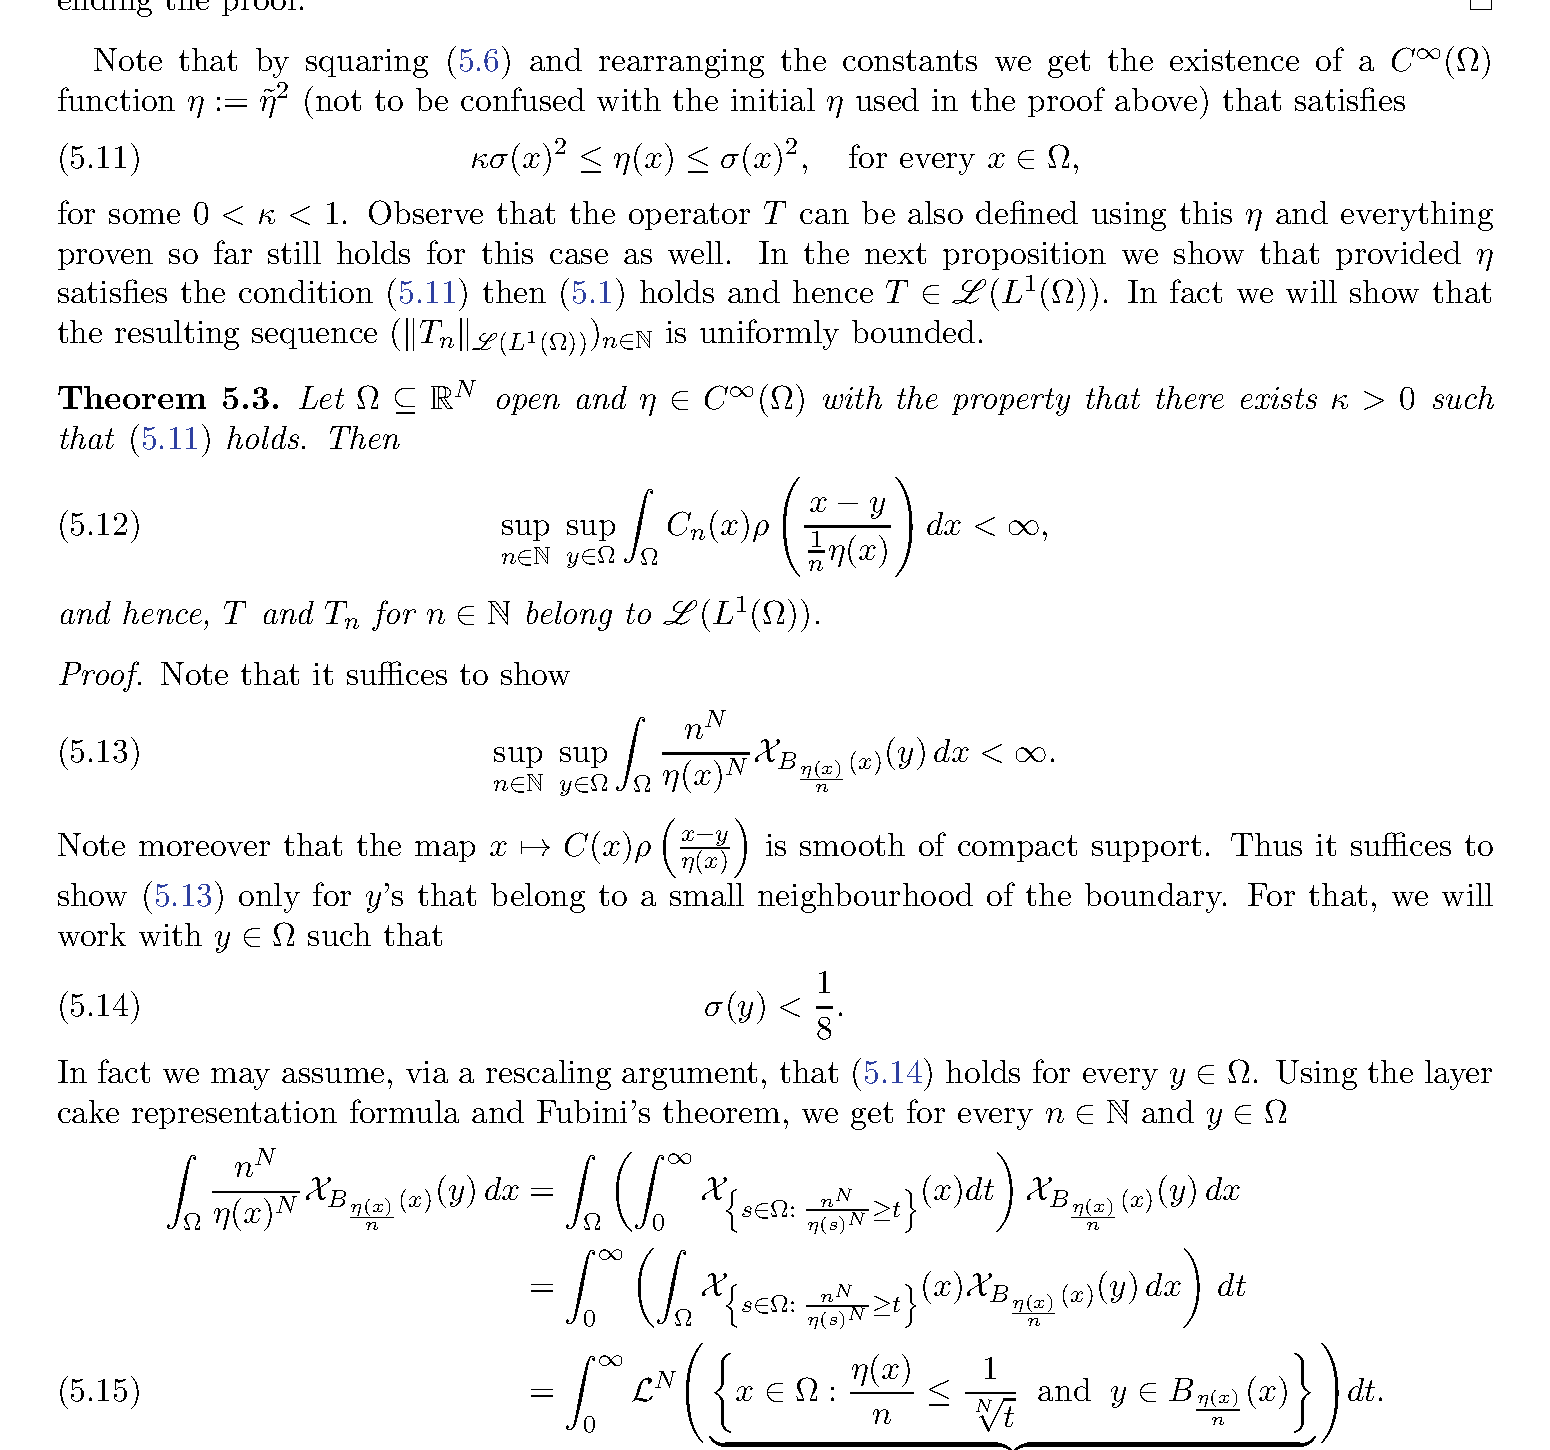
\includegraphics[width=0.95\linewidth]{figures/source_estimates_crop.png}
\end{center}

\begin{center}

\includegraphics[width=0.95\linewidth]{figures/open_problem_crop.png}
\end{center}

The exact estimate to prove is
\begin{equation}\label{eq:suff}
  \sup_{n\in\N}\sup_{y\in\Omega}
  \int_\Omega \frac{n^N}{\eta(x)^N}
  {\bf 1}_{B_{\eta(x)/n}(x)}(y)\,dx<\infty.
\end{equation}
This implies the source's estimate (5.12), because \(0\le \rho\le 1\) and
\(C_n(x)=M_\rho n^N/\eta(x)^N\).

\section*{Idea Of The Proof}

The quadratic lower bound in the source proof is used to prevent the moving
ball centered at \(x\) from seeing a fixed point \(y\) across too many
boundary scales.  A simpler mechanism is available.  If \(\eta\) has
Lipschitz constant \(L<1\), then whenever
\[
  |x-y|<\frac{\eta(x)}{n},
\]
the values \(\eta(x)\) and \(\eta(y)\) are automatically comparable:
\[
  \frac{n}{n+L}\eta(y) < \eta(x) < \frac{n}{n-L}\eta(y).
\]
Thus every relevant \(x\) lies in one ordinary ball around \(y\) of radius
comparable to \(\eta(y)/n\), and the integrand is bounded by a constant times
\(n^N/\eta(y)^N\).  Multiplying that height by that volume gives a constant
independent of \(y\), \(n\), and the boundary geometry.

\begin{theorem}[Lipschitz variable steps satisfy the \(L^1\) kernel bound]
\label{thm:main}
Let \(\Omega\subset\R^N\) be open and let
\(\eta:\Omega\to(0,\infty)\) be an \(L\)-Lipschitz function with
\(0\le L<1\).  Suppose also that
\[
  B_{\eta(x)}(x)\subset\Omega\qquad (x\in\Omega).
\]
Then
\[
  \sup_{n\in\N}\sup_{y\in\Omega}
  \int_\Omega \frac{n^N}{\eta(x)^N}
  {\bf 1}_{B_{\eta(x)/n}(x)}(y)\,dx
  \le
  \OmegaN\left(\frac{1+L}{1-L}\right)^N,
\]
where \(\OmegaN\) is the volume of the unit ball in \(\R^N\).
Consequently, for every source mollifier \(\rho\),
\[
  \sup_{n\in\N}\sup_{y\in\Omega}
  \int_\Omega C_n(x)\rho\left(\frac{x-y}{\eta(x)/n}\right)\,dx
  \le
  M_\rho\OmegaN\left(\frac{1+L}{1-L}\right)^N.
\]
In particular \(T\) and all \(T_n\) are bounded on \(L^1(\Omega)\), uniformly
in \(n\).
\end{theorem}

\begin{proof}
Fix \(n\in\N\) and \(y\in\Omega\), and set
\[
  A_{n,y}:=\{x\in\Omega:\ |x-y|<\eta(x)/n\}.
\]
If \(x\in A_{n,y}\), then the Lipschitz condition gives
\[
  \eta(x)-\eta(y)\le L|x-y|< \frac{L}{n}\eta(x),
\]
and therefore
\begin{equation}\label{eq:upper-comparable}
  \eta(x)<\frac{n}{n-L}\eta(y).
\end{equation}
Similarly,
\[
  \eta(y)-\eta(x)\le L|x-y|< \frac{L}{n}\eta(x),
\]
so
\begin{equation}\label{eq:lower-comparable}
  \eta(x)>\frac{n}{n+L}\eta(y).
\end{equation}
Equation \eqref{eq:upper-comparable} also gives
\[
  A_{n,y}\subset B_{\eta(y)/(n-L)}(y).
\]
Using \eqref{eq:lower-comparable} on \(A_{n,y}\), we obtain
\begin{align*}
  \int_\Omega \frac{n^N}{\eta(x)^N}
  {\bf 1}_{B_{\eta(x)/n}(x)}(y)\,dx
  &=
  \int_{A_{n,y}} \frac{n^N}{\eta(x)^N}\,dx \\
  &\le
  \frac{ (n+L)^N}{\eta(y)^N}
  \left|B_{\eta(y)/(n-L)}(y)\right| \\
  &\le
  \OmegaN\left(\frac{n+L}{n-L}\right)^N \\
  &\le
  \OmegaN\left(\frac{1+L}{1-L}\right)^N.
\end{align*}
This proves \eqref{eq:suff}.  The estimate with \(\rho\) follows from
\(0\le\rho\le1\) and from the formula for \(C_n\).  The \(L^1\)-boundedness
then follows exactly as in Proposition 5.1 of the source by Tonelli's theorem.
\end{proof}

\begin{corollary}[No quadratic lower bound is needed for Whitney steps]
\label{cor:whitney}
In the setting of the source with \(\Theta=\partial\Omega\), choose the
Whitney step \(\eta\) so that \(\|\nabla\eta\|_\infty\le L<1\).  Then the
source estimates (5.12) and (5.13) hold, and the \(L^1\), \(W^{1,1}\), and
the \(W^{1,1}\) conclusions, and the unmodified \(\mathrm{BV}\)
boundedness/weak-star approximation conclusions in Section 5 that used
(5.11) remain valid with this Lipschitz step in place of the quadratic step.
\end{corollary}

\begin{proof}
The source's Whitney construction already permits a harmless rescaling of
\(\eta\), and the proof of its Theorem 2.1 explicitly arranges a uniform
gradient bound below \(1\).  Since \(\eta=0\) on \(\partial\Omega\), the
bound \(\|\nabla\eta\|_\infty<1\) implies
\(\eta(x)<\dist(x,\partial\Omega)\), hence the balls \(B_{\eta(x)}(x)\) lie
inside \(\Omega\).  Theorem~\ref{thm:main} gives the missing uniform
\(L^1\) kernel estimate.  The later \(L^1\)-convergence proof, the
\(W^{1,1}\) proof, and the unmodified \(\mathrm{BV}\) weak-star proof in
the source use the quadratic condition only through that uniform \(L^1\)
bound and through boundedness of \(\nabla\eta\), both of which are now
available.
\end{proof}

\begin{remark}[Sharpness of the strict Lipschitz threshold]
The strict inequality \(L<1\) is not cosmetic.  The source's one-dimensional
example \(\Omega=(0,1)\), \(\eta(x)=\dist(x,\partial\Omega)\), has boundary
slope \(1\) and gives an unbounded \(L^1\) operator.  On the half-line model
\(\eta(x)=Lx\), the \(n=1\) kernel mass is bounded for \(L<1\) and grows like
\(\log(1/y)\) at \(L=1\).
\end{remark}

\section*{Verification Notes}

The proof is analytic.  The script
\texttt{code/verify\_lipschitz\_kernel\_bound.py} checks the exact
one-dimensional linear-step formula
\[
  \int_0^1 \frac{n}{Lx}{\bf 1}_{|x-y|<Lx/n}\,dx
\]
for several \(L<1\), compares it with the theorem's bound, and illustrates
the logarithmic growth at \(L=1\).  This is a sanity check for the geometry of
the estimate, not a substitute for the proof above.

\section*{Novelty Check And Limitations}

Cheap run indexes were searched for arXiv:1910.02751, variable-step
mollifier keywords, and the strings \texttt{eta\_bounded\_quadratic},
\texttt{integrability\_full}, and \texttt{integrability\_suff}.  No prior run
packet or attempt on this exact question was found.  A bounded web search for
the same exact strings and for close variants of ``Variable Step Mollifiers''
with ``open question'', ``quadratic'', and ``L1'' found the source article and
no later answer to this estimate.

The theorem does not claim that every possible step \(\eta<\dist(\cdot,
\partial\Omega)\) works.  The source itself gives a negative example at the
borderline boundary slope \(1\).  It also does not reprove the strict
\(\mathrm{BV}\) convergence statement for the source's separate modified
operators \(\tilde T_n\).  The result proves that the quadratic comparability
hypothesis is unnecessary for the intended Whitney-style smooth steps: a
strict Lipschitz contraction of the distance scale is enough.

\section*{Human Review Recommendation}

Review as a claimed full solution of the Section 5 open estimate in the
Whitney-step setting.  The central proof check is whether the set
\(|x-y|<\eta(x)/n\) indeed forces the two-sided comparison
\(\eta(x)\simeq\eta(y)\) with constants uniform in \(n\); the remaining
volume estimate is immediate.

\begin{thebibliography}{9}
\bibitem{HPR}
M. Hintermuller, K. Papafitsoros, and C. N. Rautenberg,
\emph{Variable step mollifiers and applications},
Integral Equations and Operator Theory 92 (2020), article 53;
arXiv:1910.02751.
\end{thebibliography}

\end{document}
